\documentclass{article}

% Four-page, double-blind ML-for-Systems workshop extended abstract.

%\usepackage[dblblindworkshop]{neurips_2026}
\usepackage[dblblindworkshop]{neurips_2026}
\usepackage{comment}

\workshoptitle{ML for Systems Workshop}

\usepackage[utf8]{inputenc}

\usepackage[T1]{fontenc}

\usepackage{hyperref}

\usepackage{url}

\usepackage{booktabs}

\usepackage{graphicx}

\usepackage{amsmath}

\usepackage{amsfonts}

\usepackage{microtype}

\usepackage{xcolor}

% This is a planning document that compiles in the conference template. Replace

% blue text as evidence becomes available; do not submit with blueprint notes.

\definecolor{blueprint}{RGB}{25,82,145}

\newcommand{\todo}[1]{\textcolor{blueprint}{[TODO: #1]}}

\newcommand{\pilot}[1]{\textcolor{blueprint}{[PILOT: #1]}}

\newcommand{\bytes}[1]{\lvert #1\rvert_{\mathrm{UTF8}}}

\newcommand{\Dec}{\operatorname{D}}
\newcommand{\Tok}{\operatorname{T}}
\newcommand{\Ser}{\operatorname{SerializeCodec}}

\title{When Adversarial Prediction Still Compresses: Tokenization and Adversarial Robustness in LLM-Based Lossless Compression}

% Tokenization Buffers Prediction Failure in LLM-Based Lossless Compression

% Keep the submission anonymous. Add authors only in the camera-ready version.

\author{Anonymous Authors}

\begin{document}

\maketitle
Large language models (LLMs) have been known to be capable of acting as powerful lossless compression machines: next-token probabilities coupled with entropy coding can substantially compress data below its raw size. Yet existing evaluations largely single out predictive performance of the LLM or at best aggregate compression ratios, leaving an important systems question understudied: \emph{when does LLM compression survive (catastrophic/worst-case) prediction failure?} We show that the answer lies in treating LLM-based compression as a two-layer system of (1) tokenization as pre-compression and (2) entropy coding with LLM-derived probabilities. On text8, Qwen2.5-0.5B compresses to $17.6\%$ of raw size, outperforming token IDs ($41.3\%$) and Brotli ($29.6\%$). Strikingly, a $5.26\times$ increase in adversarial prediction cost still yields a $31.7\%$ arithmetic-coded stream because long tokens amortize prediction errors. Removing this effect with one-byte tokens causes expansion to $119.6\%$, while conventional codecs remain compressive. 
%Tokenizer fertility therefore defines a key robustness boundary, motivating selective predictive coding with a conventional fallback.



% -----------------------------------------------------------------------------

% BLUEPRINT AT A GLANCE (delete before submission)

% Target: at most four content pages, including figures and tables. Suggested

% budget: motivation 0.75; formulation and attacks 1.0; evaluation 0.75; results

% 0.9; systems implications, limitations, and conclusion 0.6. Do not assume

% references or supplementary material are excluded from the organizers four-page

% limit; confirm their counting rule before submission.

%

% One-sentence thesis:

% Tokenization is a variable-rate front end to predictive coding, so robust

% evaluation must optimize and report code length per decoded source byte, not

% merely next-token surprisal.

%

% Claim discipline:

% (C1) Formal: token surprisal and source-normalized compression ratio are

%      different objectives whenever decoded token lengths vary.

% (C2) Method: canonical, byte-aware greedy and beam attacks directly optimize

%      entropy-floor or realized arithmetic-code expansion.

% (C3) Empirical: use only after the full multi-model/seed matrix supports it.

%      The current repository establishes a Qwen2.5-0.5B case study, not broad

%      tokenizer or model universality.

% -----------------------------------------------------------------------------

\section{Who is actually doing the heavy lifting in LLM-based compression?}

% What is doing the compression?

% Proposed Story-Line: LLM-based lossless compressors predict tokens. Arithmetic coding converts token probabilities into bits. Performance is conventionally reported using NLL or perplexity. But users store bytes, not tokens. Tokens represent unequal byte lengths. Therefore, token-level worst cases may not be compression worst cases. Your experiment reveals exactly this mismatch.

``Language Modeling Is Compression'' introduced and formalized how next-symbol probabilities can drive a lossless arithmetic coder and mentions tokenization itself as lossless precompression~\citep{deletang2024language}. This observation implies that so-called LLM compression combines two distinct mechanisms: a tokenizer replaces variable-length source strings with token IDs, and a language model predicts those IDs so that an entropy coder can shorten likely ones. That the tokenization itself already provides some compressive benefit is often under-stated and has not been systematically, jointly with LLM-based entropy compression to detangle both compressive effects studied. 

%LLMZip is another instance of this composed design~\citep{valmeekam2023llmzip}.

Prior work by Schmidt et al.~\citep{schmidt2026token} isolates the first mechanism and show that LLM token tables can themselves serve as global string dictionaries, enabling compression and operations over encoded data without model inference. Thus tokenization can be a useful compression primitive without language-model inference. This raises an attribution question for LLM codecs: how much compression comes from tokenization versus prediction?

%Schmidt et al.~\citep{schmidt2026token} isolate the first mechanism before introducing a ... . They use an LLM vocabulary as a global symbol table in which common byte strings map to fixed-width IDs and one-byte entries guarantee coverage. 

%Unlike a block-local code, this stable representation supports equality checks, hashing, joins, and aggregations before decoding. These properties make token tables particularly attractive for databases, where strings can remain encoded during common relational operations and be decoded only when needed. Thus tokenization can be a useful compression primitive without language-model inference. 

What remains unclear is how much of an LLM codec's behavior comes from this token representation and how much comes from prediction. Delétang et al. compare ASCII and BPE ~\citep{sennrich2016bpe} on natural enwik9, but the two effects have not been isolated under inputs chosen against realized end-to-end size. This matters because prediction loss is measured per token while compression is measured per source byte: a poor probability model may still sit inside a pipeline that compresses when its tokens represent many bytes, whereas low-fertility tokenization can expose expansion. We therefore study the tokenizer--predictor--coder pipeline as a two-layer system.

\paragraph{Contributions.}

We (i) factor end-to-end compression rate into tokenizer fertility and predictive coding under natural text, random input and worst-case inputs; (ii) we formalize token-, byte-, and realized-code objectives and evaluate against worst-case attacks per objective to demonstrate when the token layer absorbs predictive surprise and when it exposes expansion of the original file size and (iii) we propose a systems design for database compression that is LLM-native while still having the advantages of dictionary encodings (querabliity, ...). 

%We construct losslessly decodable adversarial inputs and separate the resulting file size into tokenizer, model, arithmetic-coder, and metadata costs.

\paragraph{Systems implication.}
The two-layer (tokenization + LLM-based entropy coding) view suggests a robust architecture for learned compression. Token IDs (global token table for all tables) can remain the stable, queryable representation used during processing, while predictive entropy coding exploiting LLM-next token probabilities is applied only as an optional storage, transport layer or to actually cold data. This separates the operational benefits of a global token representation from the inference cost and ... of the language model and introduces tokenization as LLM-native pre-compression. 
%to be determined: For near worst-case inputs, a codec can additionally store the smaller of the predictive representation and a conventional fallback, bounding expansion while retaining predictive gains on favorable inputs.


\section{Compression objectives and how to construct worst-case inputs}
\label{sec:attacks}

%TODO: shorten this paragraph, maybe put the example with hello in the appendix 
Our central distinction is between prediction difficulty and end-to-end compression failure. A token can be extremely unlikely under the language model while decoding to few source bytes. We use one notation throughout. Let $x=(x_1,\ldots,x_N)$ be the generated token sequence, let $h_t=x_{<t}$ be its token history, let $\Tok$ and $\Dec = \operatorname{decode}$ denote the tokenizer and decoder, and let $p_\theta(v\mid h)$ be the language model probability of token $v$ after history $h$. For a sequence of $N$ tokens, let $\bytes{\operatorname{decode}(x)}$ denote the number of source bytes obtained after decoding the token sequence $x$. For example, if $\operatorname{decode}(x)=\texttt{hello}$, then $\bytes{\operatorname{decode}(x)}=5$ bytes.
Define the decoded source size, in bytes, as
\begin{equation}
  B(x) = \bytes{\operatorname{decode}(x)}.
  \label{eq:source-bytes}
\end{equation}

%, so maximizing token surprisal need not maximize compressed size per input byte. We therefore evaluate three increasingly end-to-end attack objectives side by side.

Let $h$ denote the current token history and let $v$ be a candidate next token. The first objective selects the least probable next token as an extension of the series $h$, yielding the MinProb or phrased a different way MaxSurprisal objective from the set of admissible next tokens $G(h)$ from the vocabulary, %\operatorname{MinProb}(v;h)
\begin{equation}
\begin{aligned}
  v^\star_{\mathrm{tok}}
  &= \arg\min_{v\in G(h)} \left\{\log_2 p_\theta(v\mid h)\right\} \\
  &\iff \arg \max_{v\in G(h)} S_{\max}
  = \arg \max_{v\in G(h)} -\log_2 p_\theta(v\mid h)
  \qquad [\mathrm{bits/token}]
\end{aligned}
\label{eq:minprob}
\end{equation}

This is the LLM-centric token-level worst case. It maximizes ideal coded bits per token, but not necessarily bits per source byte. To account for variable-length tokenization, define the incremental decoded byte length contributed by the token $v$,
\begin{equation}
  \Delta b(v;h)=
  \bytes{\operatorname{decode}(h\mathbin\Vert v)}-
  \bytes{\operatorname{decode}(h)}.
\end{equation}
The byte-aware greedy objective then selects
\begin{equation}
  v^\star_{\mathrm{byte}} = {\arg \max}_{v\in G}
  \frac{-\log_2 p_\theta(v\mid h)}{\Delta b(v;h)}  \qquad [\mathrm{bits/byte}].
  \label{eq:spb}
\end{equation}
Unlike \ref{eq:minprob}, it directly targets the ideal entropy-coding cost per newly decoded source byte.
For a complete sequence $x$, the cumulative ideal model cost is the sequence NLL $L_\theta(x)$
\begin{equation}
  L_\theta(x)
  =
  \sum_{t=1}^{N}
  \ell_\theta(x_t\mid x_{<t})
  =
  -\sum_{t=1}^{N}\log_2 p_\theta(x_t\mid x_{<t})
  \qquad [\mathrm{bits}],
  \label{eq:nll}
\end{equation}
where any fixed initial context is implicit in $x_{<1}$. The ideal source-normalized size ratio is 
\begin{equation}
  R_{\mathrm{ideal}}(x) = 100\,\frac{L_\theta(x)}{8B(x)} \quad [\%]. \label{eq:ideal-ratio}
\end{equation}

Thus $R_{\mathrm{ideal}}<100\%$ means that the ideal predictive code is smaller than raw 8-bit source bytes.

For the realized codec, let $
  S_{\mathrm{codec}}(x)
  = \left|\Ser(x)\right|$ in bytes be the serialized output size. Its realized source-normalized size ratio is 
\begin{equation}
  R_{\mathrm{real}}(x)
  = 100\,\frac{S_{\mathrm{codec}}(x)}{B(x)}
  \quad [\%]. \label{eq:actualrate}
\end{equation}
A realized-size beam search approximately maximizes Eq.~\ref{eq:actualrate} by cloning coder state for candidate continuations. This objective captures arithmetic-coder, metadata, and framing effects that the ideal NLL does not.


\subsection{Prediction Loss Is Not Compression Loss}
\label{sec:objective-mismatch}

%TODO: find a catchy title, something that conveys that "no, prediction is not the best proxy for compression - do not forget about the tokenizer!" 

We define tokenizer fertility as
%\todo{compare fertility accross different tokenizers }
\begin{equation} f(x)=\frac{\bytes{\operatorname{decode}(x)}}{N} \qquad [\mathrm{bytes/token}], 
\end{equation}
which is average number of decoded source bytes per token. Using the sequence NLL $L_\theta(x)$, the ideal predictive rate is
\begin{equation}
  R_{\rm ideal}(x)=
  100\,\frac{L_\theta(x)}{8\bytes{\operatorname{decode}(x)}}
  =
  \underbrace{\frac{L_\theta(x)}{N}}_{\text{bits/token}}
  \underbrace{\frac{N}{\bytes{\operatorname{decode}(x)}}}_{\text{tokens/byte}}
  \frac{100}{8}.
  \label{eq:factorization}
\end{equation}
Thus high bits/token can be offset by high bytes/token. Tokenization can buffer severe prediction failure when adversarial tokens represent many source bytes. Hence, there is a compression boundary (ignoring finite coder state, metadata overhead, etc.) that occurs at $\frac{L(x)}{N} < 8\,\frac{\bytes{\operatorname{decode}(x)}}{N} = 8 f(x) $. Thus the break-even prediction cost grows linearly with tokenizer fertility.
A token representing $f$ source bytes can tolerate up to $8f$ bits of
surprisal before the predictive layer expands the source.

%Thus, a tokenizer with fertility f bytes/token can absorb up to 8f bits/token of prediction cost.

%(This is the robustness mechanism we test:)


\subsection{Token-, Byte-, and Codec-Level Attacks}
% Adversarial model and generation policies

We assume white-box access to the compression pipeline: the adversary can inspect the tokenizer, model logits, and coding algorithm when
constructing an input and construct length-$N$ adversarial inputs by autoregressive search over a candidate alphabet $G$ using different scoring functions. To ensure that generated token sequences survive decoding and retokenization, every prefix must satisfy, $T(\operatorname{decode}(x_{1:t}))=x_{1:t}$ as final decoding must recover exactly the same IDs and bytes (see appendix for more information on canonical decoding). 

We compare three generation policies that we benchmark against natural text from wikipedia (text8 in UTF-8) and random string sequences as baselines: 
\emph{Minimum probability} greedily maximizes Eq.~\ref{eq:minprob}. \emph{Maximum surprisal/byte} greedily maximizes Eq.~\ref{eq:spb}. \emph{Realized-size beam} searches over multiple canonical continuations to approximately maximize Eq.~\ref{eq:actualrate}.

%\emph{Natural text} is the non-adversarial corpus baseline. %\emph{Random canonical} uniformly samples valid canonical extensions and controls for unusual token sequences without optimizing against the model.


%TODO: I do not yet know how to include this / where to best put it. 

%The \emph{one-byte UTF-8 ablation} is not a separate attack objective. It is an ablation of the candidate alphabet in which $G$ contains only canonical tokens contributing one decoded byte. This fixes fertility near one byte/token and removes the multi-byte-token buffering mechanism. Under an exact one-byte constraint, MinProb and SurprisalPerByte induce the same greedy ranking.

The \emph{one-byte UTF-8 ablation} restricts the candidate alphabet $G$ to canonical tokens representing exactly one decoded byte, thereby removing variation in token fertility. Under this constraint, the multi-byte buffering is removed and MinProb and SurprisalPerByte induce the same greedy ranking.

%TODO: think about if this can be shorted or removed. If it stays, call the masking + rescoring an optimization of LLM-based compression. 
\paragraph{(Global mask re-scoring as an optimization} 
When evaluating occurring-token dictionaries, we construct each adversarial sequence once under the full distribution and replay identical IDs and histories under the post-hoc occurring-token mask. This isolates probability renormalization; it is not a mask-adaptive attack.) - tbd if I will include it

\section{Experimental design}
\label{sec:design}

\paragraph{Setup.}
We evaluate Qwen2.5-0.5B on natural text, random canonical input, canonical full-vocabulary adversarial sequences, and a one-byte UTF-8 ablation. Each input in the primary attack evaluation contains 10,000 tokens, except for the explicitly marked preliminary surprisal-per-byte smoke test. All attacks use the same model, context, and arithmetic-coding configuration, and generated prefixes must round-trip through tokenizer decoding and re-encoding. Table~\ref{tab:decisive} reports the primary token-budget results. Figure~\ref{fig:layered_compression_robustness} separately compares complete codecs on byte-matched prefixes; its exact values are retained as an auxiliary table in Appendix~\ref{tab:codec-comparison}.

\paragraph{Reported quantities.}
For every primary input or attack, we report prediction cost $L_\theta(x)/N$ (bits/token), tokenizer fertility $B(x)/N$ (bytes/token), ideal model cost per source byte, arithmetic-coder payload cost per source byte, and $R_{\mathrm{AC}}(x)=100\,S_{\mathrm{AC}}(x)/(8B(x))$. These primary-table quantities exclude QACS container metadata. Figure~\ref{fig:layered_compression_robustness} instead reports the complete-stream ratio $R_{\mathrm{real}}$. Values below $100\%$ denote compression relative to raw UTF-8, while values above $100\%$ denote expansion. Unavailable production-scale measurements are shown with an em dash.

\begin{table}[t]

\centering

\caption{
\textbf{Source-normalized predictive coding under increasingly adverse inputs.} Token-level surprisal / LLM prediction cost alone is not predictive of compression failure. Arrows indicate the direction favorable to compression ($\downarrow$ lower is better; $\uparrow$ higher is better). AC size $R_{\mathrm{AC}}$ reports the arithmetic-coder payload relative to raw UTF-8; $^\dagger$ Preliminary 32- and 128-token smoke tests only (three seed runs each).
$^\ddagger$ Preliminary 1,024-token smoke test (one seed run).
}

\label{tab:decisive}

\small
\setlength{\tabcolsep}{3.2pt}

\begin{tabular}{lrrrrr}

\toprule

\multicolumn{1}{l}{Input / condition} &
\multicolumn{1}{c}{Prediction cost $\downarrow$} &
\multicolumn{1}{c}{Tokenizer fertility $\uparrow$} &
\multicolumn{1}{c}{Ideal predictive rate $\downarrow$} &
\multicolumn{1}{c}{AC payload rate $\downarrow$} &
\multicolumn{1}{c}{AC size $R_{\mathrm{AC}}$ $\downarrow$} \\

\multicolumn{1}{l}{} &
\multicolumn{1}{c}{\footnotesize (bits/token)} &
\multicolumn{1}{c}{\footnotesize (bytes/token)} &
\multicolumn{1}{c}{\footnotesize (bits/byte)} &
\multicolumn{1}{c}{\footnotesize (bits/byte)} &
\multicolumn{1}{c}{\footnotesize (\% of raw)} \\

\midrule

\multicolumn{6}{l}{\textit{Baselines}} \\

Natural text (text8, UTF-8)
    & 5.11
    & 5.59
    & 0.92
    & 1.13
    & $14{,}1\%$ \\

Random canonical (UTF-8)
    & 8.74
    & 1.30
    & 6.71
    & 7.59
    & $94{,}8\%$ \\

\midrule

\multicolumn{6}{l}{\textit{Adversaries}} \\

MinProb adversary
    & $26.86 \pm 0.05$
    & $7.09 \pm 0.04$
    & $3.79 \pm 0.02$
    & $2.53 \pm 0.01$
    & $31{,}7 \pm 0{,}2\%$ \\

Max. surprisal/byte ($N=32$)$^\dagger$
    & $19.26 \pm 0.39$
    & $1.45 \pm 0.02$
    & $12.89 \pm 0.40$
    & $10.74 \pm 0.31$
    & $134{,}2 \pm 3{,}9\%$ \\

Max. surprisal/byte ($N=128$)$^\dagger$
    & $17.82 \pm 0.13$
    & $1.48 \pm 0.01$
    & $11.96 \pm 0.07$
    & $10.43 \pm 0.06$
    & $130{,}4 \pm 0{,}7\%$ \\

Max. surprisal/byte ($N=1024$)$^\ddagger$
    & $17.49 \pm 0.00$
    & $1.47 \pm 0.00$
    & $11.87 \pm 0.00$
    & $10.50 \pm 0.00$
    & $131{,}3 \pm 0{,}0\%$ \\

Realized-size beam
    & --- & --- & --- & --- & --- \\

\midrule

\multicolumn{6}{l}{\textit{Tokenizer ablation}} \\

One-byte UTF-8 ablation
    & $8.33 \pm 0.00$
    & $1.00 \pm 0.00$
    & $8.33 \pm 0.00$
    & $9.57 \pm 0.00$
    & $119{,}6 \pm 0{,}0\%$ \\

\bottomrule

\end{tabular}

\end{table}

\section{Results}
\label{sec:results}

\begin{figure}[t]
    \centering
    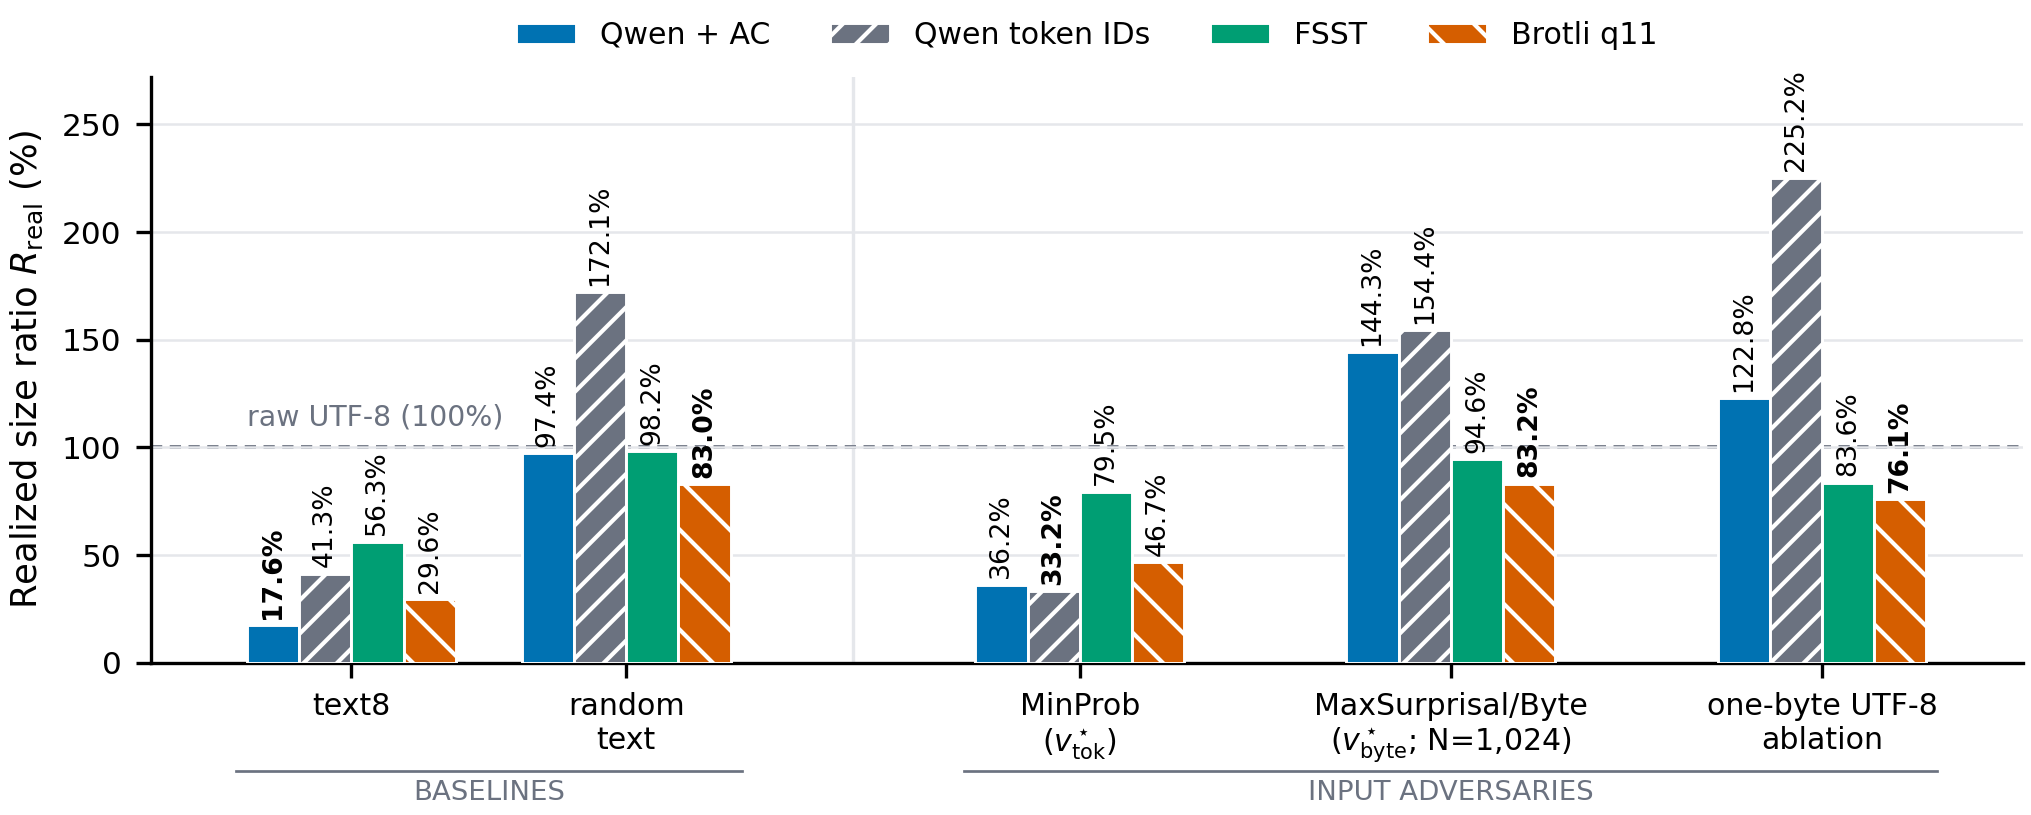
\includegraphics[width=\linewidth]{plots/end_to_end_compressor_robustness.png}
    \caption{\textbf{End-to-end compression across natural and adversarial inputs.}
    Realized size ratio $R$ for complete Qwen+AC, fixed-width Qwen token-ID,
    FSST, and Brotli streams. The dashed line marks raw UTF-8 ($R=100\%$);
    lower is better, and bold values mark the smallest complete stream for each
    input. The MinProb adversary greedily selects the least-probable canonical
    continuation. The 10,000-token full-vocabulary MaxSurprisal/Byte result is
    pending. Shared Qwen model weights and the tokenizer table are excluded from
    both Qwen representations.}
    \label{fig:layered_compression_robustness}
\end{figure}


\paragraph{Natural text versus distribution shift. (interpretation of first two datasets in barplot)}
As expected, prediction provides large gains on natural text: on text8,
Qwen+AC reaches $R=17{,}6\%$, compared with $41{,}3\%$ for fixed-width token
IDs and $29{,}6\%$ for Brotli. Under distribution shift introduced by the randomly 
created text, this advantage largely disappears. On random printable text, 
Qwen+AC reaches $R=98{,}2\%$, while Brotli reaches $83{,}0\%$ and the token-ID 
representation expands to $R=172{,}8\%$. The token-ID representation expanding to 
$R=172{,}8\%$ (vs. $R=98{,}2\%$ for Qwen+AC) thus shows that prediction recovers much 
of a poor representation (this needs more investigation).

%Thus prediction can substantially repair an inefficient token representation without necessarily yielding a competitive compressor.

\paragraph{Prediction failure does not imply compression failure. (interpretation of the MinProb adversary result)}
The 10,000-token minimum-probability attack raises prediction cost to
$26.86\pm0.05$ bits/token, $5.26\times$ the text8 value of $5.11$ bits/token.
Nevertheless, its tokens decode to $7.09\pm0.04$ source bytes/token, so the
large token-level surprisal corresponds to only $3.79$ ideal bits/byte
($R_{\mathrm{ideal}}=47{,}4\%$). The arithmetic-coder payload is smaller still
at $2.53\pm0.01$ bits/byte, or $R_{\mathrm{AC}}=31{,}7\pm0{,}2\%$. The
finite-frequency coder floors extremely small probabilities, so this gap from
the unquantized model estimate is a quantization effect rather than improved
prediction. In the auxiliary byte-matched comparison, the complete Qwen+AC
stream remains compressive at $R=36{,}2\%$, although fixed-width token IDs are
slightly smaller at $R=33{,}2\%$. This shows that under the MinProb attack,
robustness to prediction failure comes primarily from the multi-byte token
representation rather than from an additional predictive-coding gain.

\paragraph{Removing tokenizer fertility exposes predictive expansion. (interpretation of the one-byte UTF-8 ablation and the max. suprisal/byte result)}
The one-byte UTF-8 ablation removes this buffering mechanism by fixing fertility
at one byte/token. Its ideal cost rises to $8.33$ bits/byte
($R_{\mathrm{ideal}}=104{,}1\%$), already beyond the raw-byte break-even point
predicted by Eq.~\ref{eq:factorization}, while the arithmetic-coder payload
reaches $9.57$ bits/byte ($R_{\mathrm{AC}}=119{,}6\%$). The auxiliary
byte-matched comparison shows the same end-to-end failure: complete Qwen+AC
expands to $R=122{,}8\%$, whereas Brotli remains compressive at $76{,}1\%$.
Together with the MinProb result, this isolates tokenizer fertility as the
mechanism that allows severe token-level prediction errors to remain
source-level compression. The ablation establishes this mechanism, but not the
globally strongest attack; unrestricted full-vocabulary surprisal-per-byte and
realized-size searches remain future measurements. Finally, complete-stream
overhead is non-negligible at these block sizes: across the five auxiliary
inputs, seed, dictionary, configuration, and framing add 331--334 bytes, with
text8 increasing from a $14{,}3\%$ arithmetic payload to a $17{,}6\%$
complete stream. Reporting only entropy or payload would therefore overstate 
realized compression, especially on small blocks.


\section{Results (old)}
\label{sec:results}

\paragraph{Prediction helps strongly on natural text, but not under distribution shift.} %TODO: this is kind of trivial. Of course Qwen+AC will work best on natural text, you can shorten this paragraph and introduce it with "As expected, ..."
On text8, Qwen+AC attains $R=17{,}6\%$ ($5.68\times$ compression), compared with $41{,}3\%$ for fixed-width token IDs, $29{,}6\%$ for Brotli, and $56{,}3\%$ for FSST. Prediction therefore reduces the token-ID representation by $57{,}4\%$ and yields a stream $40{,}5\%$ smaller than Brotli. On random printable text, however, Qwen+AC only reaches $R=98{,}2\%$, while Brotli reaches $83{,}0\%$. The token-ID representation expands to $R=172{,}8\%$, showing that prediction recovers much of a poor representation without producing a competitive compressor.

\paragraph{Prediction failure does not imply compression failure.}
The 10,000-token minimum-probability attack reaches $26.86\pm0.05$ bits per predicted token, $5.26\times$ the text8 value of 5.11 bits/token. Yet its tokens decode to $7.09\pm0.04$ source bytes/token, yielding 3.79 ideal bits/byte ($R_{\mathrm{ideal}}=47{,}4\%$). Its arithmetic-coder payload rate is $2.53\pm0.01$ bits/byte, or $R_{\mathrm{AC}}=31{,}7\pm0{,}2\%$. The finite-frequency coder floors extremely small probabilities, so realized arithmetic length can be lower than the unquantized model estimate; this is a coder-quantization effect, not unexpectedly accurate prediction. In the auxiliary matched-byte comparison, token IDs reach $R=33{,}2\%$ and the complete Qwen+AC stream reaches $R=36{,}2\%$.

\paragraph{Removing tokenizer fertility exposes predictive expansion.}
The one-byte UTF-8 ablation fixes fertility at one byte/token. Table~\ref{tab:decisive} shows an ideal cost of 8.33 bits/byte ($R_{\mathrm{ideal}}=104{,}1\%$) and an arithmetic-coder payload cost of 9.57 bits/byte ($R_{\mathrm{AC}}=119{,}6\%$). Thus, once multi-byte tokens cannot amortize model surprise, the predictive layer crosses the raw-byte break-even point predicted by Eq.~\ref{eq:factorization}. The auxiliary codec comparison shows the same qualitative failure on a byte-matched prefix of this input: complete Qwen+AC reaches $R=122{,}8\%$, while Brotli remains at $76{,}1\%$. This controlled ablation establishes the mechanism, but not the globally strongest attack; unrestricted full-vocabulary surprisal-per-byte and realized-size searches remain future measurements.

\section{System Implications - Designing LLM Compression That Fails Gracefully}

%Systems implications and limitations


\label{sec:limitations}

The systems lesson is to preserve token IDs as the global, queryable in-memory representation and treat predictive arithmetic coding as an optional block-level storage or transport layer. 

Source-normalized accounting identifies whether fragility comes from the tokenizer, predictor, quantizer, dictionary, or container.

For high-cost input blocks (meaning ones with data-model mismatch), a guard can store the smaller of predictive and conventional encodings plus a selector bit, bounding size by the fallback plus one bit; its decoding granularity, latency, and throughput remain to be measured.


%TODO: rephrase this limitations paragraph
%Our evidence is limited to one model, synthetic white-box inputs, three starts, finite context, approximate search, and one coder/container. It does not establish global worst cases or generalize to multilingual text or code. The attack could enable storage or compute amplification; practical mitigations include size caps, early-abort expansion detection, bounded inference, and fallback codecs.

\section{Conclusion}

Robust learned compression is an end-to-end systems problem. The full-vocabulary token-level attack is $5.26\times$ harder to predict than text8 yet still has an arithmetic-coder payload ratio of $R_{\mathrm{AC}}=31{,}7\%$ because long tokens buffer that surprise. Under the one-byte UTF-8 ablation, removing this buffer causes the complete Qwen+AC stream to expand to $122{,}8\%$ of raw UTF-8, while conventional codecs remain below the raw size. A practical learned codec should therefore measure realized source-normalized cost and fall back to a conventional encoding when prediction ceases to help.

\begin{ack}

\todo{Camera-ready only: funding and competing-interest disclosures. The supplied style hides this environment in anonymous submission mode.}

\end{ack}

\bibliographystyle{plainnat} % use the style required by the workshop/template
\bibliography{references}


\newpage
\section{Appendix}


\paragraph{Why canonicality is required.}
Not every sequence of valid token IDs can arise from tokenizing its own decoded
bytes. For example, suppose the vocabulary contains tokens for
\texttt{a}, \texttt{b}, and \texttt{ab}. The token sequence
$[\texttt{a},\texttt{b}]$ decodes to \texttt{ab}, but the tokenizer may encode
\texttt{ab} as the single token $[\texttt{ab}]$. Hence, decoding and
retokenizing changes the token sequence. Since our attacks select token IDs
directly from the model distribution, allowing such sequences would optimize
over token histories that cannot occur for the corresponding source input.
We therefore require every generated partial sequence to be canonical, i.e.,
$T(\operatorname{decode}(x_{1:t}))=x_{1:t}$.



\subsection{Experimental details}
\label{app:experimental-details}

\paragraph{Model and coder.}
We use Qwen2.5-0.5B with 151,643 non-special candidate tokens, a context length of 1,000 tokens, 100 retained context tokens between coding blocks, and KV caching. The arithmetic coder uses a 32-bit state and a frequency total of 262,144. The finalized QACS version-1 stream records the seed, model and coder configuration, token count, raw byte count, arithmetic payload, any required token dictionary, and framing. Model weights and the shared tokenizer table are treated as shared decoder state and excluded from both Qwen representations.

\paragraph{Inputs and aggregation.}
Every production sequence in the primary attack evaluation contains 10,000 tokens. Table~\ref{tab:decisive} reports natural text, random canonical input, the full-vocabulary minimum-probability attack, and the one-byte UTF-8 ablation under this common token budget; the maximum-surprisal-per-byte row is populated only by a marked 32-token smoke test, and the missing realized-size measurement is left blank. Attack statistics are means and sample standard deviations over three independent canonical seed runs.

Figure~\ref{fig:layered_compression_robustness} and Appendix Table~\ref{tab:codec-comparison} are a separate codec-level diagnostic. For that comparison only, we serialize representative prefixes with 9,996--10,000 decoded source bytes so that complete-stream sizes are directly comparable across codecs. Thus Table~\ref{tab:decisive} reports arithmetic payload ratio $R_{\mathrm{AC}}$ for the token-budget runs, whereas the figure reports complete-stream $R_{\mathrm{real}}$ for byte-matched prefixes.

All generated prefixes satisfy
\[
\Tok(\Dec(x_{1:t}))=x_{1:t}, \qquad t=1,\ldots,N,
\]
and every final stream is independently decoded back to identical token IDs and UTF-8 bytes. FSST uses the official implementation at commit \texttt{e638d4cf8c26129d73c242a4127b42b975de5b63}; Brotli uses quality~11; token IDs use a fixed 18-bit representation with a stream header.

\paragraph{Cost accounting.}
In the auxiliary codec comparison, we report both the Qwen+AC arithmetic payload and the complete serialized stream. Their difference is 331--334 bytes across the five byte-matched inputs. The finite-frequency table reserves a nonzero count for every vocabulary entry, so extremely small model probabilities are clipped. Consequently, realized arithmetic length can be lower than unquantized NLL on the minimum-probability attack; this quantization effect is reported rather than interpreted as predictive accuracy.

\paragraph{Layered compression robustness and cost attribution.} \textbf{(a)} End-to-end size relative to raw UTF-8, separating fixed-width token IDs, the ideal model surprisal cost, the realized arithmetic-coding (AC) payload plus dictionary metadata, and the final serialized file (dot). The serialized size can be decomposed as ($S_{\mathrm{total}} = S_{\mathrm{payload}} + S_{\mathrm{dict}} + S_{\mathrm{frame}}$), where $S_{\mathrm{payload}}$ is the finalized arithmetic payload, $S_{\mathrm{dict}}$ is dictionary metadata, and $S_{\mathrm{frame}}$ is the remaining container and framing overhead.

\begin{table}[t]
\centering
\caption{\textbf{Realized size ratio by input and codec.} Values are encoded bytes divided by raw UTF-8 bytes and reported as percentages; lower is better. AC payload excludes the Qwen container and is shown only for cost attribution. All entries in the four codec columns are complete, round-trip-verified streams, and bold marks the smallest complete stream per row.}
\label{tab:codec-comparison}
\small
\setlength{\tabcolsep}{3.4pt}
\begin{tabular}{lrrrrr}
\toprule
Input & AC payload & Qwen+AC & Token IDs & FSST & Brotli \\
\midrule
text8                    & $14.3\%$ & \textbf{$17.6\%$} & $41.3\%$ & $56.3\%$ & $29.6\%$ \\
Random printable         & $94.8\%$ & $97.4\%$ & $172.1\%$ & $98.2\%$ & \textbf{$83.0\%$} \\
MinProb ($\vtok$) adversary         & $32.9\%$ & $36.2\%$ & \textbf{$33.2\%$} & $79.5\%$ & $46.7\%$ \\
MaxSurprisal/Byte ($\vbyte$; $N=1{,}024$) & $122.4\%$ & $144.3\%$ & $154.4\%$ & $94.6\%$ & \textbf{$83.2\%$} \\
One-byte UTF-8 ablation & $119.5\%$ & $122.8\%$ & $225.2\%$ & $83.6\%$ & \textbf{$76.1\%$} \\
\bottomrule
\end{tabular}
\end{table}


The printable-only row is retained solely as an alphabet-sensitivity check: restricting the candidate set to the 95 printable ASCII bytes weakens, but does not remove, predictive expansion.


\paragraph{Tokenizer fertility stats}

\begin{table}[t]
  \centering
  \small
  \caption{Tokenizer fertility on the held-out 5\,MB text8 test region
  (855{,}233 whitespace-delimited words). The text8 BPE is trained only on the
  first 90\,MB with a 32k vocabulary. Fertility is tokens per word (lower is
  better); bytes per token is the compression-oriented inverse (higher is
  better). All tokenizers reconstruct the input exactly. The domain-trained BPE
  produces 4.4\% fewer tokens than Qwen.}
  \label{tab:tokenizer-fertility}
  \begin{tabular}{@{}lrrrrr@{}}
    \toprule
    Tokenizer & Vocab. & Used & Tokens & Tok./word $\downarrow$ & Bytes/tok. $\uparrow$ \\
    \midrule
    ASCII byte & 128 & 27 & 5{,}000{,}000 & 5.8464 & 1.0000 \\
    text8 BPE (32k) & 32{,}000 & 26{,}617 & 933{,}499 & \textbf{1.0915} & \textbf{5.3562} \\
    Qwen2.5 & 151{,}665 & 25{,}798 & 976{,}828 & 1.1422 & 5.1186 \\
    \bottomrule
  \end{tabular}
\end{table}




\paragraph{Reported quantities.}
The primary and auxiliary evaluations share the same token- and source-normalized quantities but differ in stream accounting:

\begin{align}
  \text{Bits/token} &= \frac{L_\theta(x)}{N},\\
  \text{Bytes/token} &= \frac{\bytes{\operatorname{decode}(x)}}{N},\\
  \text{Ideal bits/byte} &= \frac{L_\theta(x)}
    {\bytes{\operatorname{decode}(x)}},\\
  \text{AC bits/byte} &= \frac{S_{\mathrm{AC}}(x)}
    {\bytes{\operatorname{decode}(x)}},\\
  R_{\mathrm{AC}} &= 100\,\frac{S_{\mathrm{AC}}(x)}
    {8\,\bytes{\operatorname{decode}(x)}},\\
  R_{\mathrm{real}} &= 100\,\frac{\left|\operatorname{SerializeCodec}(x)\right|}
    {\bytes{\operatorname{decode}(x)}} \quad [\%].
\end{align}

Both ratios are relative to raw UTF-8; $R<100\%$ denotes compression and $R>100\%$ denotes expansion.


% Supplementary planning notes (do not count toward the four-page narrative):

% - Prove the token/byte objective mismatch and give attack pseudocode.

% - Record configurations, revisions, commands, seeds, hardware, compute, and

%   licenses; report full per-run tables and search-budget ablations.

% - Document exact seed-token, quantization, bitmap, payload, and header costs.

% - Repository map: src/adversarial.py; src/compression\_attacks.py;

%   scripts/run\_compression\_attacks.py; evaluation/notebooks/neurips/

%   adversarial\_worst\_case.ipynb; and artifacts/runs/adversarial/

%   qwen\_05b\_ascii\_bytes\_n1000.

% - Confirm whether references and the NeurIPS checklist are outside the

%   organizers four-page limit. Keep the checklist unless organizers explicitly

%   say their workshop does not require it.


%TODOS:

% put idea in there that tokenization is base-compression and then llm based compression can be used on top of that. This ensures that we can still query some of the content (please read tokenization compression paper again).

% include classical baselines such as brotli, llmzip

% include tokenization only as baseline and report for different tokenizers (Qwen’s large vocabulary;, a smaller BPE tokenizer; ideally a byte-level or byte-fallback baseline)

% mention FSST and include it as baseline 

% cite the econimics of LLM based compression from Andreas Kipf 



\end{document}
